%!TEX root = report.tex

This chapter discusses the back-end. This includes the REST API plus the database storing all the statistics data. We will first discuss the technologies that where used to build these component then how together these technologies and components form the back-end.

\section{Technology Stack}
\label{sec:2:technologyStack}
In this section we will describes as in section \ref{sec:1:technologyStack} what technologies where used and why we decided to used these above others.

\subsection{Flask}
\label{ssec:2:flask}
Flask \cite{flask} is a python micro framework for the web. Flask is based on Werkzeug \cite{werkzeug} and Jinja2 \cite{jinja2}. We have used the Flask framework as a base, but mostly used it's extensions described below. We choose Flask for our back-end because one of us already had some experience with Flask and both of us had worked (a little bit) with python before.

\subsubsection{Extensions}
To make our development easier we decided to use already existing solutions for building a REST API using Flask and MongoDb (\autoref{ssec:2:mongodb}). In this section we will describe the used extensions.

\begin{description}

\item[Flask-Restful] s an extension for Flask that adds support for quickly build- ing REST APIs. It is a lightweight abstraction that can work together with existing ORM/libraries. Because Flask-RESTful \cite{flask-restful} encourages best practices with minimal setup we were able to build a qualitatively good REST with reasonable ease.

\item[Flask-MongoKit] is and extension that builds on the Python Pymongo extension \cite{pymongo} and Flask. MongoKit adds an easy way to define MongoDb database models/documents \cite{flask-mongokit}.
\end{description}

\subsection{MongoDB}
\label{ssec:2:mongodb}
MongoDB (from``humongous'') is an open-source, document based, NoSQL database with a lot of cool features, we list a few of these that were important for the choice for MongoDB over other NoSQL database solutions \cite{mongo-db}.

\begin{description}
\item[Replication \& High Availability] A replica set in MongoDB is a group of mongod processes that maintain the same data set. Replica sets provide redundancy and high availability, and are the basis for all production deployments. Because of this feature and the requirement for the project to be fault tolerant we found this to be a positive point for choosing MongoDB. The actual implementation of this feature in our project will be discussed in \autoref{sssec:2:replication}.

\item[Map/Reduce] MongoDB provides an easy way to use map/reduce functionality. The map and reduce function can be written in JavaScript. In the Flask back-end it is very easy to apply these function to the database. This functionality was a requirement for the project and will be discussed in \autoref{sssec:2:mapreduce}.
\end{description}

\subsection{HAProxy}
\label{ssec:2:haproxy}
From the website of HAProxy \cite{ha-proxy}. HAProxy is a free, very fast and reliable solution offering high availability, load balancing, and proxying for TCP and HTTP-based applications. It is particularly suited for very high traffic web sites and powers quite a number of the world's most visited ones. Over the years it has become the de-facto standard opensource load balancer, is now shipped with most mainstream Linux distributions, and is often deployed by default in cloud platforms.

HAProxy is a load balancing solution pointed out by one of the student assistants and we chose to use this because it is according to their website the default solution for any professional cloud platform and beside fairly easy to set up. We will discuss HAProxy further in \autoref{sssec:2:loadbalancing}.

\section{Design}

This section describes the design of the back-end of the STALKER project. 

\subsection{Database}
Because API calls to the social media API's are done in the frontend (see \autoref{sec:1:design}) the back-end only has to worry about the statistics. We will first describe the database models. Below a list of descriptions of the used terminology is provided. In \autoref{fig:2:datamodel} we give a more detailed overview of the data models.

\begin{description}
\item[Stalker] A person who uses the STALKER application to search other people.
\item[Victim] A person who is being searches and is marked by the Stalker as the person he/she wanted to find.
\item[Search] This stores the link between a stalker, search and a victim.
\end{description}

\begin{figure}
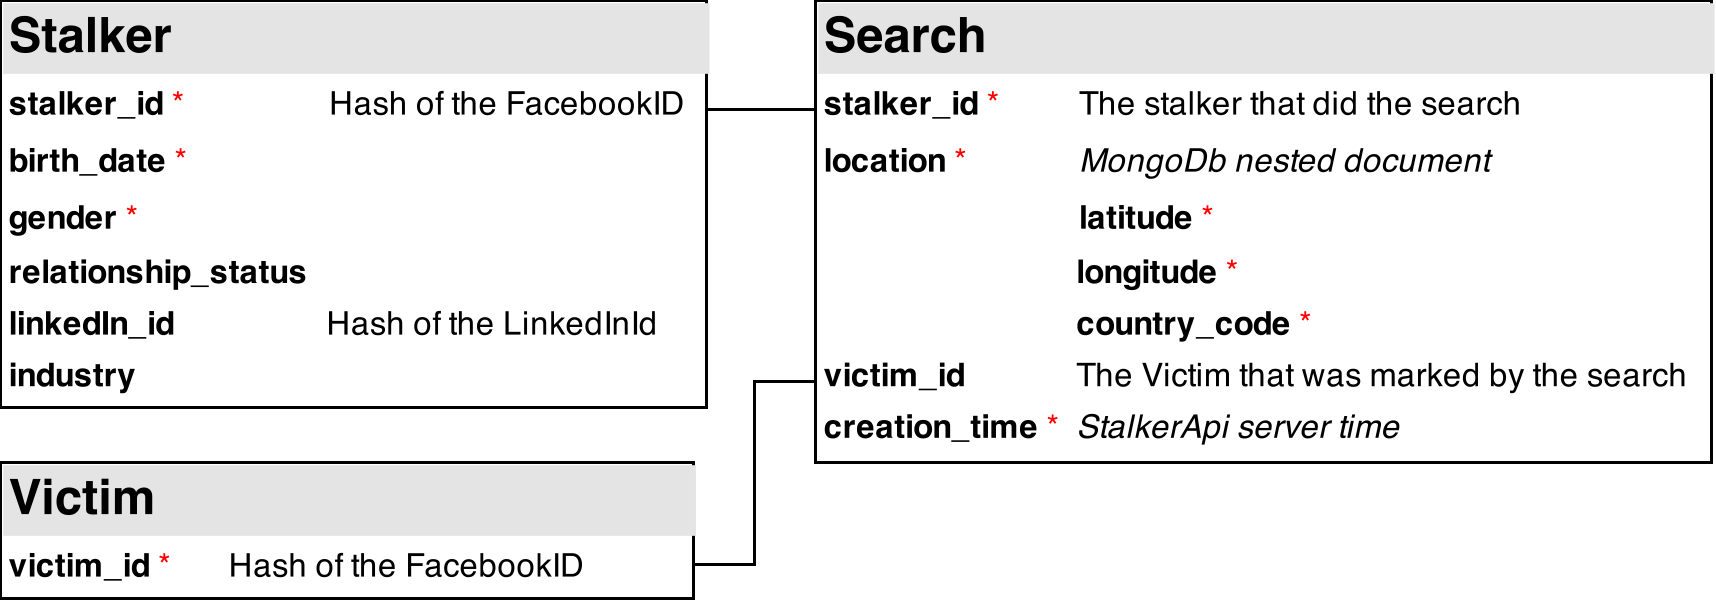
\includegraphics[width=\textwidth]{./img/database_models}   
\caption{A overview of the database models. The attributes that are required and should be always available are marked with the red *. Not all information is available from the social media API's.}
\label{fig:2:datamodel}
\end{figure}

The statistics are generated with the map reduce methods described in \autoref{sssec:2:mapreduce}.

\subsubsection{Map Reduce}
\label{sssec:2:mapreduce}
Map-reduce is a paradigm invented by google and is inspired by the functional programming functions map and reduce. The map-reduce method thus consists of a map function which performs filtering and sorting of the data. The reduce method then performs a summary operations and in our case reduces the data to some nice statistic. 

Example of map-reduce in our project. When the front-end requests a statistic e.g. the number of searches done per location. The map function will filter the data stored in the collection that stores the searches and will emit per search every location with a count of one. The reduce function will then reduce this list of locations into a list of unique locations. The reduce function does this by merging (taking the sum of) the counts when encountering double locations, this has as result a list of unique location and the number of searches done from those locations. This statistic is then shown in the front-end see \autoref{fig:1:viewStat}.

\subsubsection{Replication}
\label{sssec:2:replication}
This section describes a way MongoDB handles replication, see the image shown in \autoref{fig:2:replicationset}. All write calls from the REST API (see \autoref{ssec:2:restapi}) to the database are done to the primary MongoDb instance. This data is then replicated to the secondary instances (That run on different machines). Read operation can be load balanced to any of the instances. 

\begin{figure}
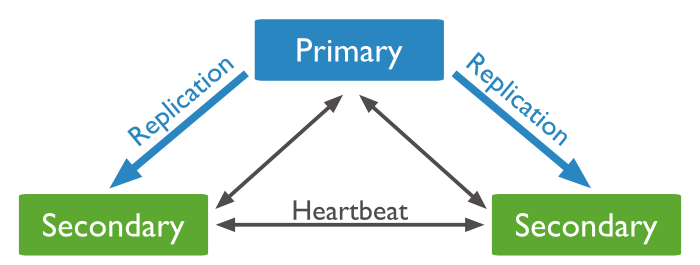
\includegraphics[width=\textwidth]{./img/replica_set}   
\caption{Replication implementation MongoDB}
\label{fig:2:replicationset}
\end{figure}

All instances know of the other instances and send heartbeat message to each other to ensure this. Whenever the other detect the primary stopped running they decide which one of them becomes the new primary (the first secondary that receives a majority votes becomes the new primary). When you have three database instances you can handle one faulty instance, so if another one stops the communication between the database and REST Api is gone. 

We chose for three databases because this number was according to the MongoDB website more than enough replication for most problems. Plus this number of processes was still manageable on our development environments.

\subsection{REST API}
\label{ssec:2:restapi}
This section describes the part of the back-end that implements all the server calls and is the part that does the communication with the database(s). We chose to build a REST Api because it is a stateless architecture which gives it good performance and scalability properties. It is very easy to run multiple instances of a REST Api, because it does not know anything about the previous requests and does not store a state.

% Please add the following required packages to your document preamble:
% \usepackage[table,xcdraw]{xcolor}
% If you use beamer only pass "xcolor=table" option, i.e. \documentclass[xcolor=table]{beamer}
\begin{table}[ht]
\begin{tabularx}{\textwidth}{rXX}
\hline
\multicolumn{3}{l}{\cellcolor[HTML]{C0C0C0}\textbf{Stalker REST API Specification}} \\ \hline
\multicolumn{1}{l}{\textit{Resource + methods}} & \textit{Input} & \textit{Output} \\ \hline
\multicolumn{3}{l}{\cellcolor[HTML]{EFEFEF}/searches} \\ \hline
GET &  & Returns: A list of JSON Search objects \\ \hline
POST & Input: JSON Search object* & Returns: The id of the created Search object \\ \hline
\multicolumn{3}{l}{\cellcolor[HTML]{EFEFEF}/search/\textless string:id\textgreater} \\ \hline
PUT & Input: JSON object with victim\_id and in the url a search id & Info: Updates a search object \\ \hline
\multicolumn{3}{l}{\cellcolor[HTML]{EFEFEF}/stalkers} \\ \hline
GET &  & Returns: A list of JSON Stalker objects \\ \hline
POST & Input: JSON Stalker object* &  \\ \hline
\multicolumn{3}{l}{\cellcolor[HTML]{EFEFEF}/victims} \\ \hline
GET &  & Returns: A list of JSON victim objects \\ \hline
POST & Input: JSON vicim object* &  \\ \hline
\multicolumn{3}{l}{\cellcolor[HTML]{EFEFEF}/statistics/location/frequency} \\ \hline
GET & Info: Counts searches per locationa & Returns: A list of JSON location frequency objects \\ \hline
\multicolumn{3}{l}{\cellcolor[HTML]{EFEFEF}/statistics/relationship/frequency} \\ \hline
GET & Info: Counts the relationships of stalkers who search & Returns: A list of JSON relationship frequency objects \\ \hline
\multicolumn{3}{l}{\cellcolor[HTML]{EFEFEF}/statistics/gender/relationship/frequency/\textless string:gender\textgreater} \\ \hline
GET & Input: Male/Female & Returns: A list of JSON gender relationship objects \\ \hline
\multicolumn{3}{l}{\cellcolor[HTML]{EFEFEF}/statistics/gender/location/frequency} \\ \hline
GET & Info: Males/Females followed by a list of locations & Returns: A list of JSON gender location objects \\ \hline
\end{tabularx}
\end{table}

\subsubsection{Load balancing}
\label{sssec:2:loadbalancing}
The REST Api can be run on different machine and load balanced using HAProxy. This proces is best described using an image, this image is included in figure \ref{fig:2:haproxy}. HAProxy knows about all the api servers and when it gets a request for the REST service it will send the request to one of the three (in our case) REST services running.

\begin{figure}
\centering
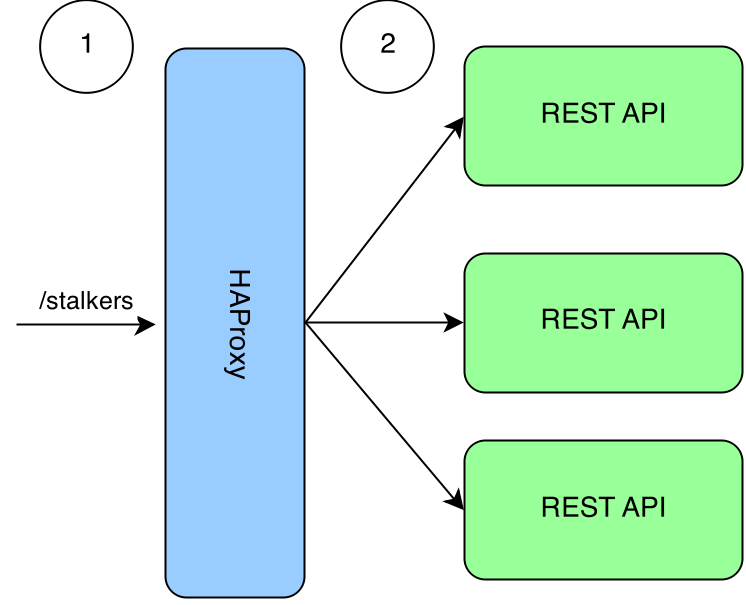
\includegraphics[height=6cm]{./img/haproxy}  
\caption{This image shows the structure of what HAProxy does.}
\label{fig:2:haproxy}
\end{figure}

If one of the REST service stops this is not a problem for HAProxy and it will keep sending the requests to the other machines. Because the services are REST services it doesn't matter if first a create POST for a search was done on server x and the update of that same search was done to another server y. This illustrates the power of the stateless web services.

\subsection{Overview}
When we combine all the back-end elements. We get an image like the image in \autoref{fig:2:overview}
\begin{figure}
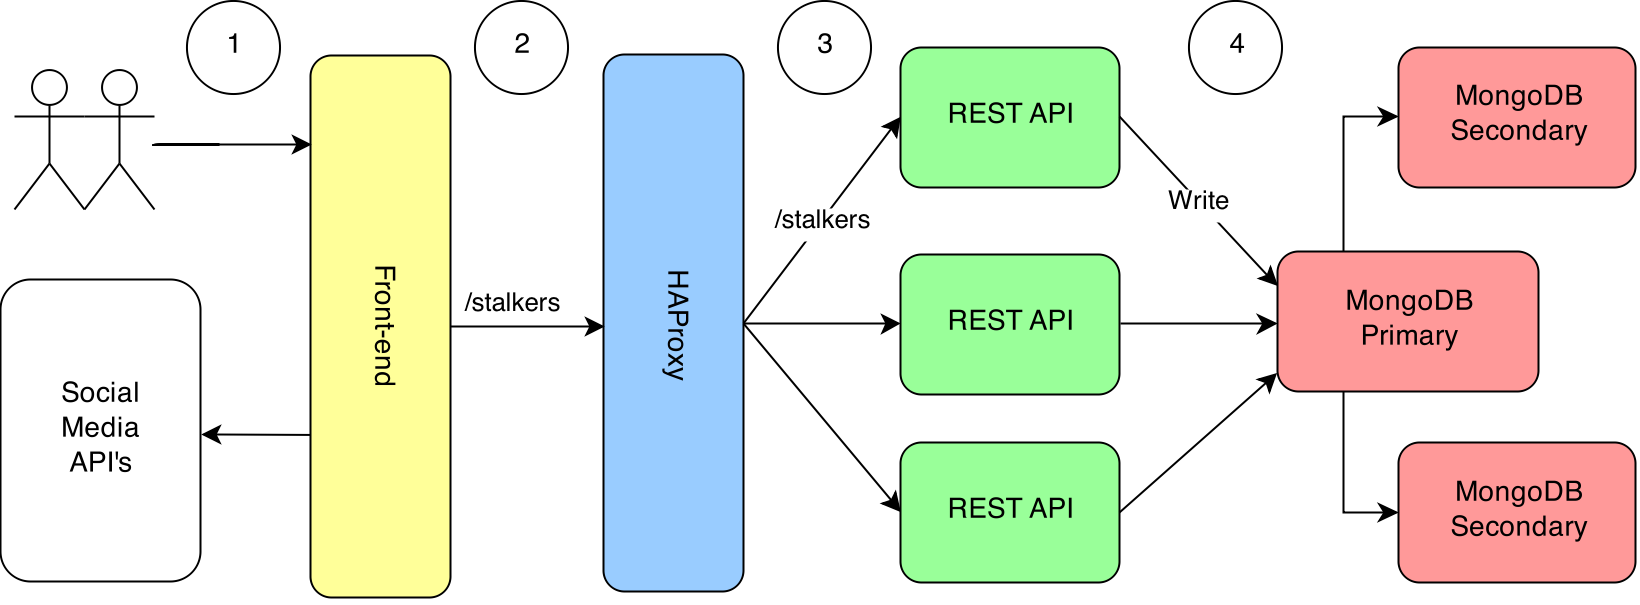
\includegraphics[width=\textwidth]{./img/overview} 
\caption{A schematic overview of the control flow when a user logs in.}
\label{fig:2:overview}
\end{figure}
